\documentclass{article}
\usepackage[utf8]{inputenc}

\title{EE2703 Applied Programming Lab \\   Assignment 9}  
\author{
  \textbf{Name}: Neham Hitesh Jain\\
  \textbf{Roll Number}: EE19B084
}\date{May 8, 2021}

\usepackage{listings}
\usepackage{natbib}
\usepackage{geometry} % Used to adjust the document margins
\usepackage{amsmath}
\usepackage{subfig}
\usepackage{verbatim}
\usepackage{color}
\usepackage{graphicx}
\definecolor{dkgreen}{rgb}{0,0.5,0}
\definecolor{gray}{rgb}{0.5,0.5,0.5}
\definecolor{mauve}{rgb}{0.58,0,0.82}

\lstset{frame=tb,
  language=Python,
  aboveskip=3mm,
  belowskip=3mm,
  showstringspaces=false,
  columns=flexible,
  basicstyle={\small\ttfamily},
  numbers=none,
  numberstyle=\tiny\color{gray},
  keywordstyle=\color{blue},
  commentstyle=\color{dkgreen},
  stringstyle=\color{mauve},
  breaklines=true,
  breakatwhitespace=true,
  tabsize=3
}

\geometry{verbose,tmargin=1in,bmargin=1in,lmargin=1in,rmargin=1in}

\begin{document}

\maketitle
\newpage

\begin{abstract}

    In this assignment, we continue our analysis of signals using Fourier
    Transforms. This time, we focus on finding transforms of functions which
    are discontinuous when periodically extended. An example of this is
    \(\sin(\sqrt{2} t)\). The discontiuity causes fourier components in
    frequencies other than the sinusoids frequency which decay as
    \(\frac{1}{\omega}\), due to Gibbs phenomenon. We resolve this problem
    using the process of windowing. In this assignment, we focus on one
    particular type of window - the Hamming window. We use this windowed
    transform to analyse signals known to contain a sinusoid of unknown
    frequencies and extract its phase and frequency. We then perform a
    sliding DFT on a chirped signal and plot a spectrogram or a
    time-frequency plot.    

\end{abstract}

\section{Assignment Examples}

The worked examples in the assignment are given below: \\ \\
\noindent
Spectrum of $sin(\sqrt{2}t)$ is given below: \newline
\begin{figure}[!tbh]
\centering
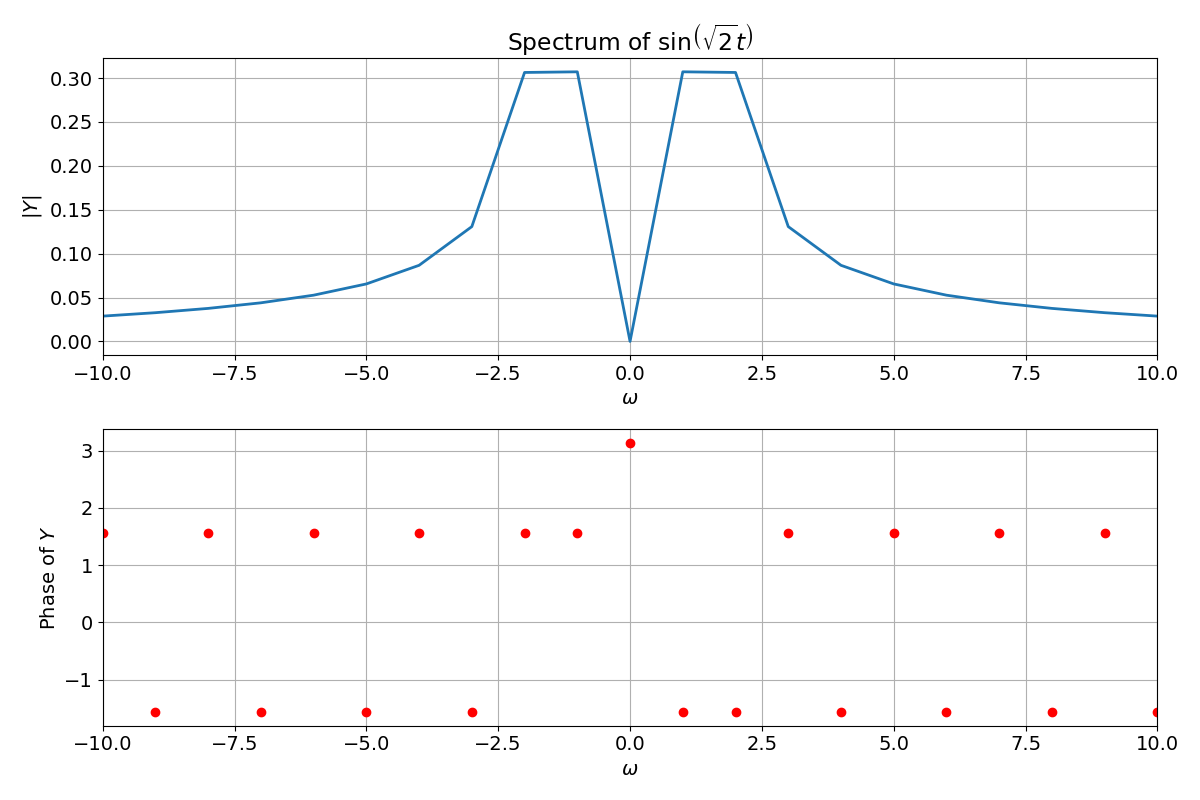
\includegraphics[scale=0.4]{plots/sin(sqrt(2).png}
\caption{Spectrum of $sin(\sqrt{2}t)$}
\label{fig:1}
\end{figure}
\newpage
Original function for which we want the DFT to be calculated:
\begin{figure}[!tbh]
\centering
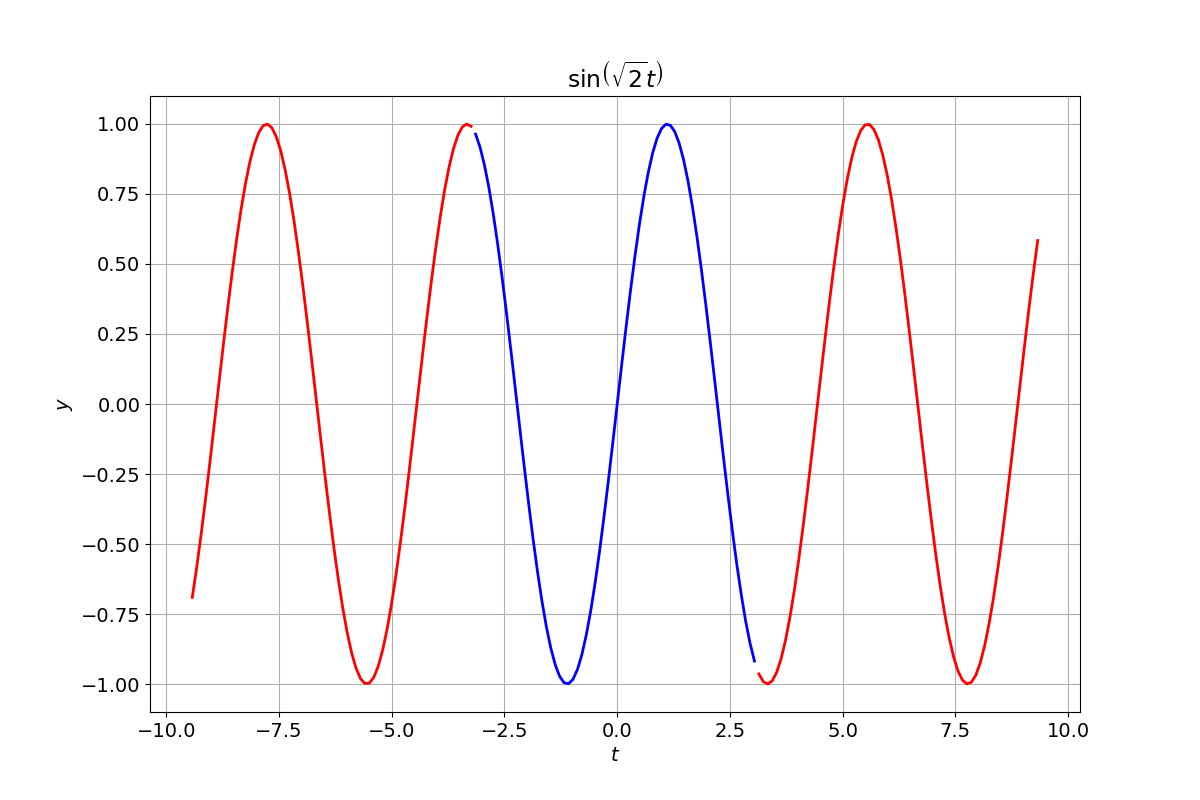
\includegraphics[scale=0.4]{plots/sin(sqrt(2)_plot.png}
\caption{$sin(\sqrt{2}t)$}
\label{fig:2}
\end{figure}
\noindent
\\
However, when we calculate the DFT by sampling over a finite time
window, we end up calculating the DFT of the following periodic signal:

\begin{figure}[!tbh]
\centering
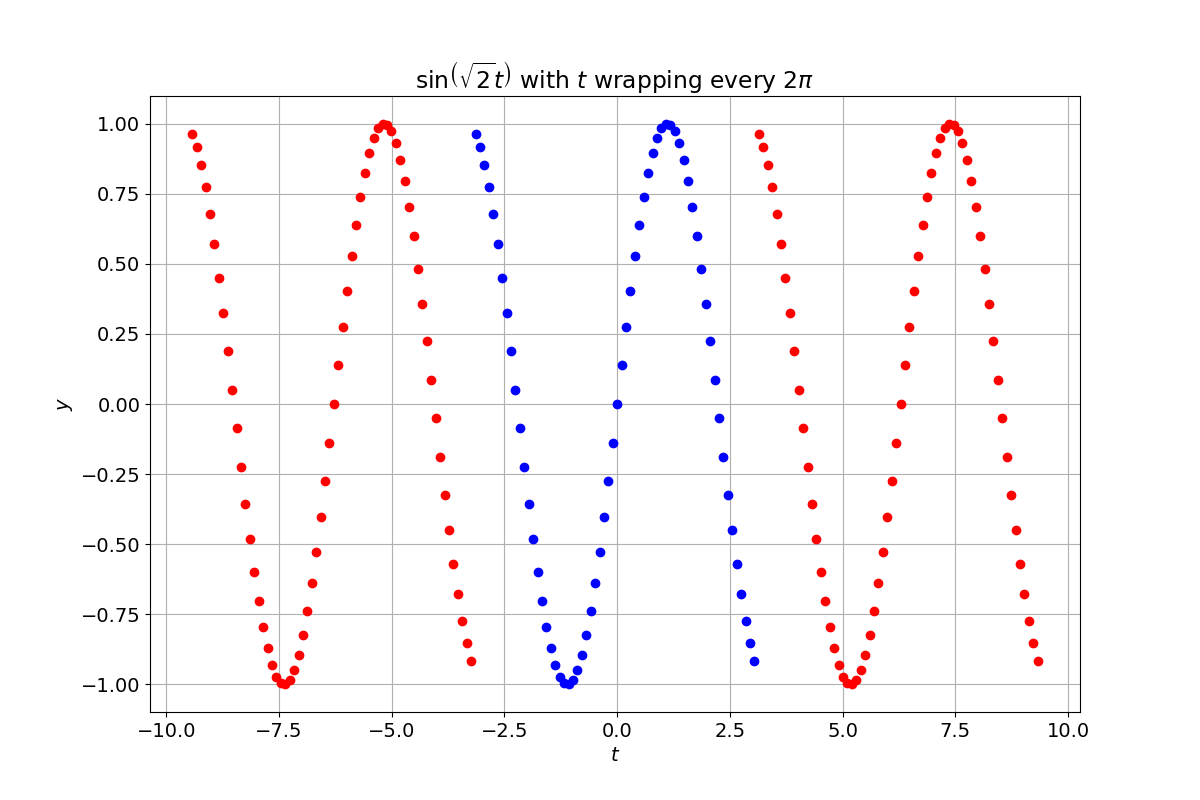
\includegraphics[scale=0.4]{plots/wrapped_sin.png}
\caption{Wrapped $sin(\sqrt{2}t)$}
\label{fig:3}
\end{figure}

These discontinuities lead to  non harmonic components in the FFT which decay as \(\frac{1}{\omega}\). To confirm
this, we plot the spectrum of the periodic ramp below:
\begin{figure}[!tbh]
\centering
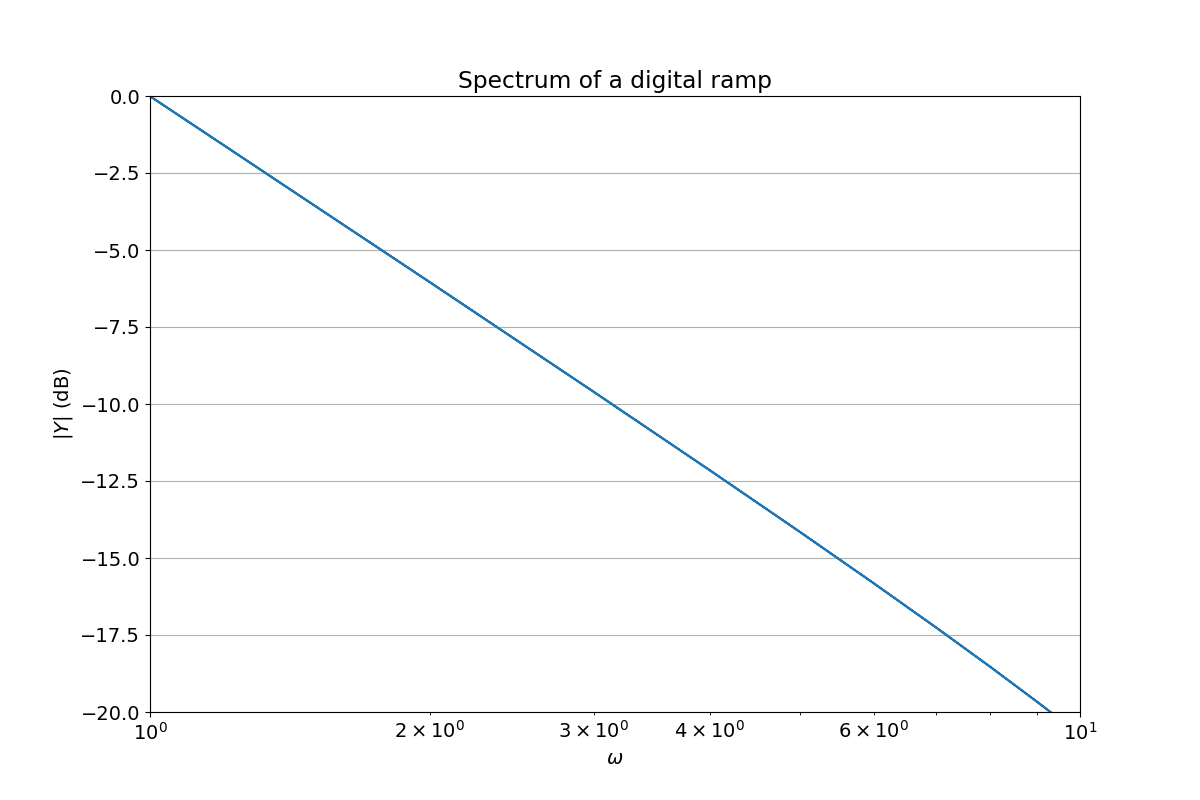
\includegraphics[scale=0.4]{plots/ramp.png}
\caption{Spectrum of ramp function}
\label{fig:4}
\end{figure}

\subsection{Hamming Window}
The hamming window removes discontinuities by attenuating the high frequency components that cause the discontinuities.
The hamming window function is given by
\begin{equation}
    x[n] = 0.54 + 0.46*cos(\frac{2\pi n}{N-1})
\end{equation}

\noindent
We now multiply our signal with the hamming window and periodically extend it. Note that the discontinuities nearly vanish
\begin{figure}[!tbh]
\centering
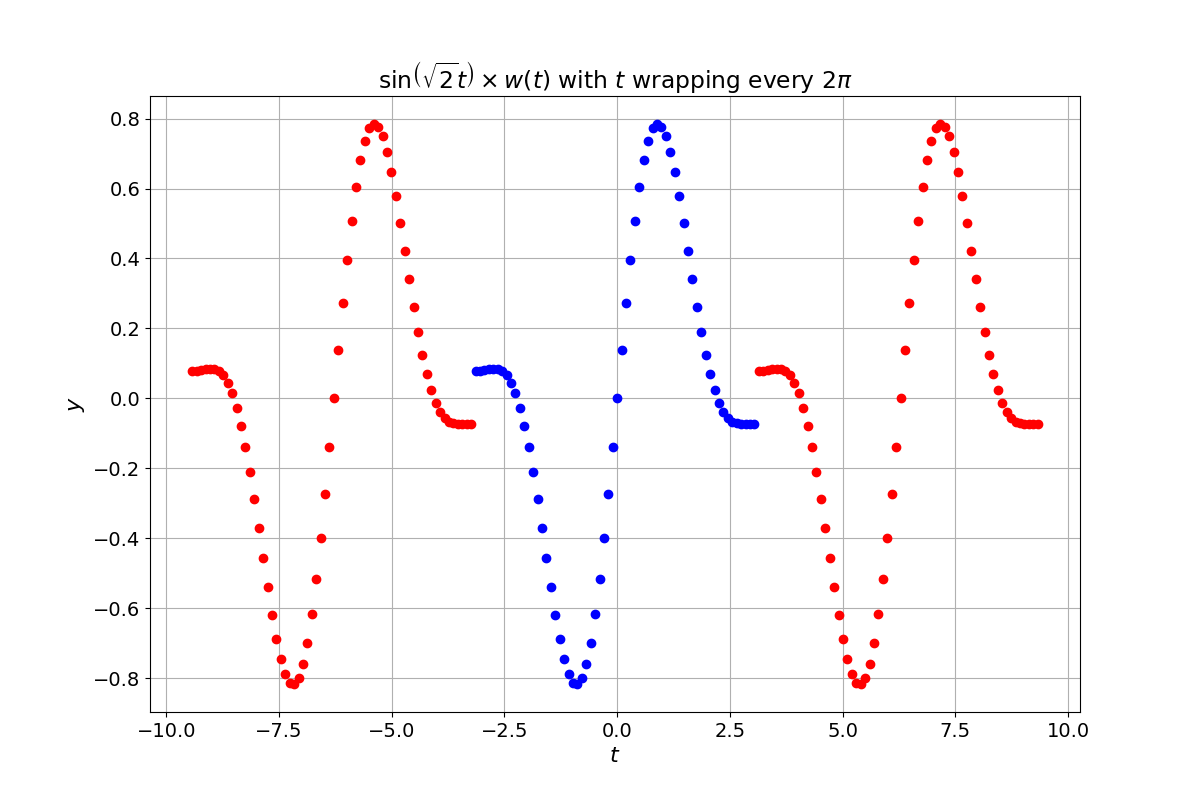
\includegraphics[scale=0.4]{plots/windowed_sin.png}
\caption{$sin(\sqrt{2}t)$ multiplied with Hamming Window}
\label{fig:5}
\end{figure}


\subsection{General Function to Calculate the Fast Fourier Transform}

We first write a general function to find the FFT of a given
input signal. Using the parameters we can control whether we want windowing in
the function or not.

\begin{lstlisting}

def calculate_fft(lim,n,f,t_,t_lims,windowing,xlim1,title1,xlabel1, ylabel2,savename,semilog):
    
    if(t_lims):
        t = t_
    else:
        t=linspace(-lim,lim,n+1)[:-1]
    dt=t[1]-t[0]
    fmax=1/dt
    y = f(t)
    if (windowing):
        m=arange(n)
        wnd=fftshift(0.54+0.46*cos(2*pi*m/n))
        y = y*wnd

    y[0]=0 # the sample corresponding to -tmax should be set zeroo
    y=fftshift(y) # make y start with y(t=0)
    Y=fftshift(fft(y))/float(n)
    w=linspace(-pi*fmax,pi*fmax,n+1)[:-1]
    
    mag = abs(Y)
    ph = angle(Y)
    
    if semilog:
        p2=General_Plotter(xlabel1,ylabel1,ylabel2,title1,savename)
        p2.semilog(abs(w),20*log10(abs(Y)),1,10,-20,0)

    else:
        if plot_flag:
            p1=General_Plotter(xlabel1,ylabel1,ylabel2,title1,savename)
            p1.plot_fft(w,mag,ph,xlim1)

    return w,Y

\end{lstlisting}

\clearpage

\subsection{Spectrum of $sin(\sqrt{2}t)$ using Hamming Window} 

The spectrum that is obtained with a time period $2\pi$ is given below:

\begin{figure}[!tbh]
\centering
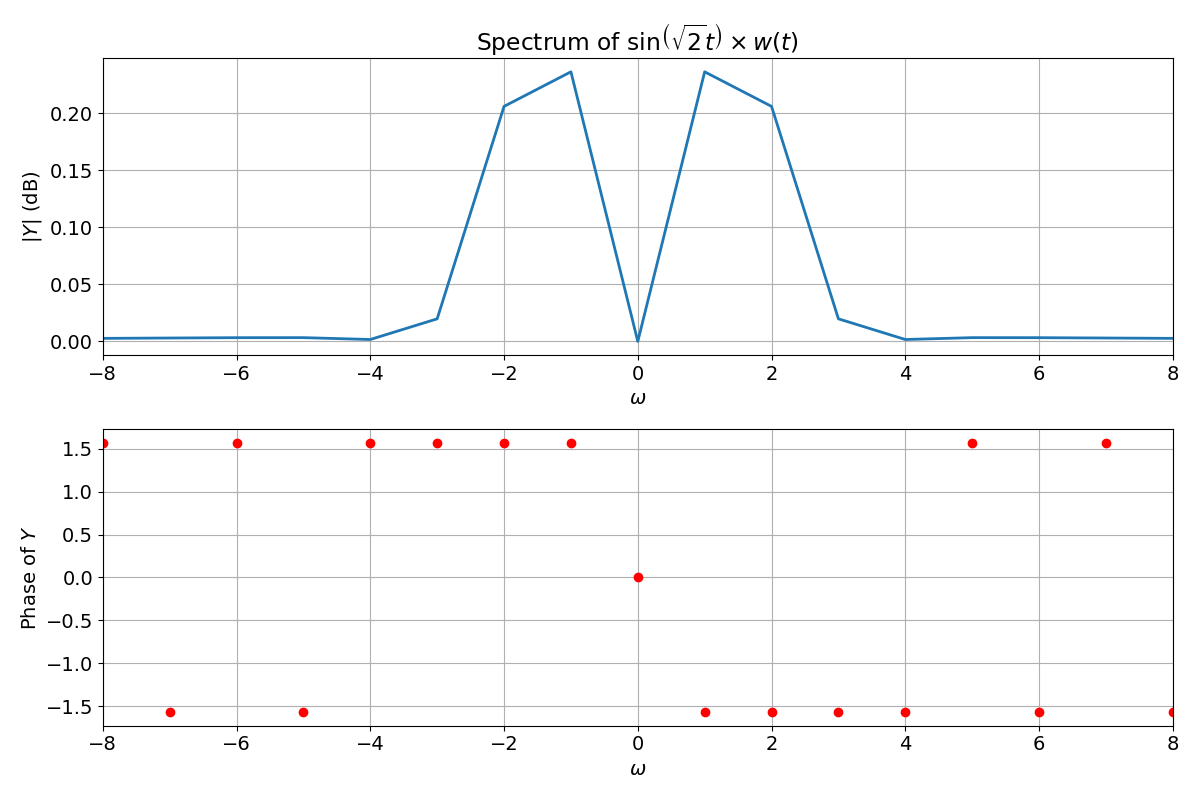
\includegraphics[scale=0.4]{plots/sin_sqrt2_window1.png}
\caption{Spectrum of $sin(\sqrt{2}t)*w(t)$ with limit $2\pi$}
\label{fig:6}
\end{figure}

The spectrum that is obtained with a time period $8\pi$ has a slightly sharper peak and is given below:


\begin{figure}[!tbh]
\centering
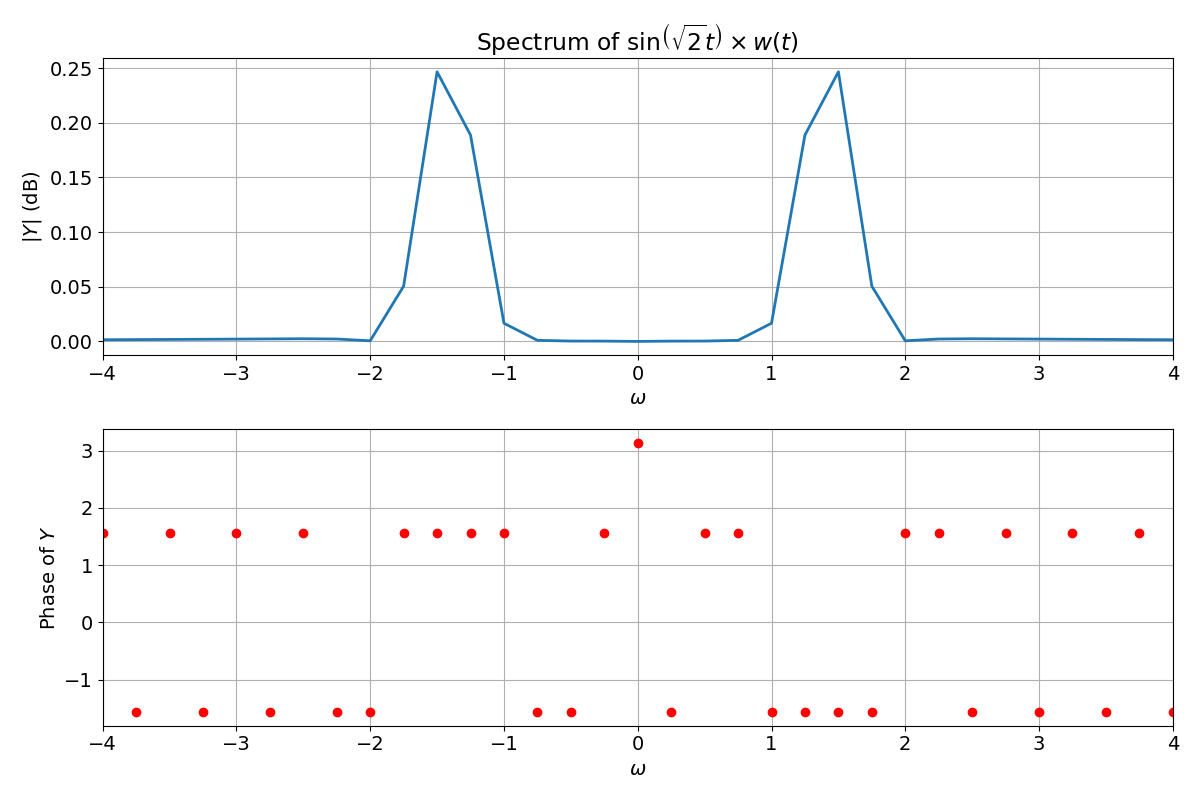
\includegraphics[scale=0.4]{plots/sin_sqrt2_window2.png}
\caption{Spectrum of $sin(\sqrt{2}t)*w(t)$ with limit $8\pi$}
\label{fig:7}
\end{figure}


\begin{itemize}
    \item
      We observe that in the case without a Hamming window, a lot of energy
      in the spectrum was in frequencies other than those of the signal.
      This is because of the Gibbs phenomenon.
    \item
      We observe that the windowed transform is much better in terms of the
      magnitude spectrum. Only components near the frequencies of the input
      signal are present, while others are mostly 0. The reason that some
      frequencies near the actual peak are present is because multiplying by
      a window in the time domain corresponds to a convolution in the
      frequency domain with its fourier transform. This means that the delta
      functions in the frequency domain are smeared out by the spectrum of
      the Hamming window.
\end{itemize}
    
    

\section{Assignment questions}

\subsection{Plotter Function}
Given below is a helper function that helps us plot.

\begin{lstlisting}
#Helper Class for Plotting the Fourier Transforms
class General_Plotter():
    ''' Class used for plotting different plots. Shortens the code by quite a bit'''
    
    fig_num=0   #Defined static variable for the figure number
    def __init__(self,xlabel1,ylabel1,ylabel2=None,title1=None,save_name=None):
        ''' xlabel,ylabel,title are used in every graph''' 

        self.xlabel1 = xlabel1
        self.ylabel1 = ylabel1
        
        self.xlabel2 = xlabel1
        self.ylabel2 = ylabel2
        
        self.title1=title1

        self.save_name=save_name
        self.fig=plt.figure(self.__class__.fig_num)
        self.__class__.fig_num+=1

    def general_funcs1(self,ax,xlim,ylim):
        ''' General functions for every graph'''
        
        ax[0].set_ylabel(self.ylabel1)
        ax[0].set_xlabel(self.xlabel1)
        ax[0].set_title(self.title1)
        ax[1].set_ylabel(self.ylabel2)
        ax[1].set_xlabel(self.xlabel2)
        if xlim is not None:
            ax[0].set_xlim(-xlim,xlim)
            ax[1].set_xlim(-xlim,xlim)
        if ylim is not None:
            ax[1].set_ylim(-ylim,ylim)

        plt.grid(True)
        plt.tight_layout()
        #plt.show()
        self.fig.savefig("plots/"+self.save_name+".png")
        close()
    
    def general_funcs2(self,ax):
        ''' General functions for every graph'''
        
        ax.set_ylabel(self.ylabel1)
        ax.set_xlabel(self.xlabel1)
        ax.set_title(self.title1)
        self.fig.savefig("plots/"+self.save_name+".png")
        close()
    
    def general_plot(self,x1,y1,mark):
        axes=self.fig.add_subplot(111)
        axes.plot(x1,y1,mark)
        self.general_funcs2(axes)

    def semilog(self,x,y,xlim1,xlim2,ylim1,ylim2):
        
        axes=self.fig.add_subplot(111)
        axes.semilogx(x,y)
        axes.set_xlim(xlim1,xlim2)
        axes.set_ylim(ylim1,ylim2)
        self.general_funcs2(axes)

    def plot_fft(self,w,mag,phi,xlim=None,ylim=None):
        ''' Helper Function for plotting the fft of a given signal'''
        
        axes=self.fig.subplots(2,1)
        axes[0].plot(w,mag,lw=2)
        axes[1].plot(w,phi,'ro')
        self.general_funcs1(axes,xlim,ylim)

\end{lstlisting}



\subsection{Question 2}

In this question, we shall plot the FFT of $cos^3(0.86t)$
The FFT without the hamming Window:
\begin{figure}[!tbh]
\centering
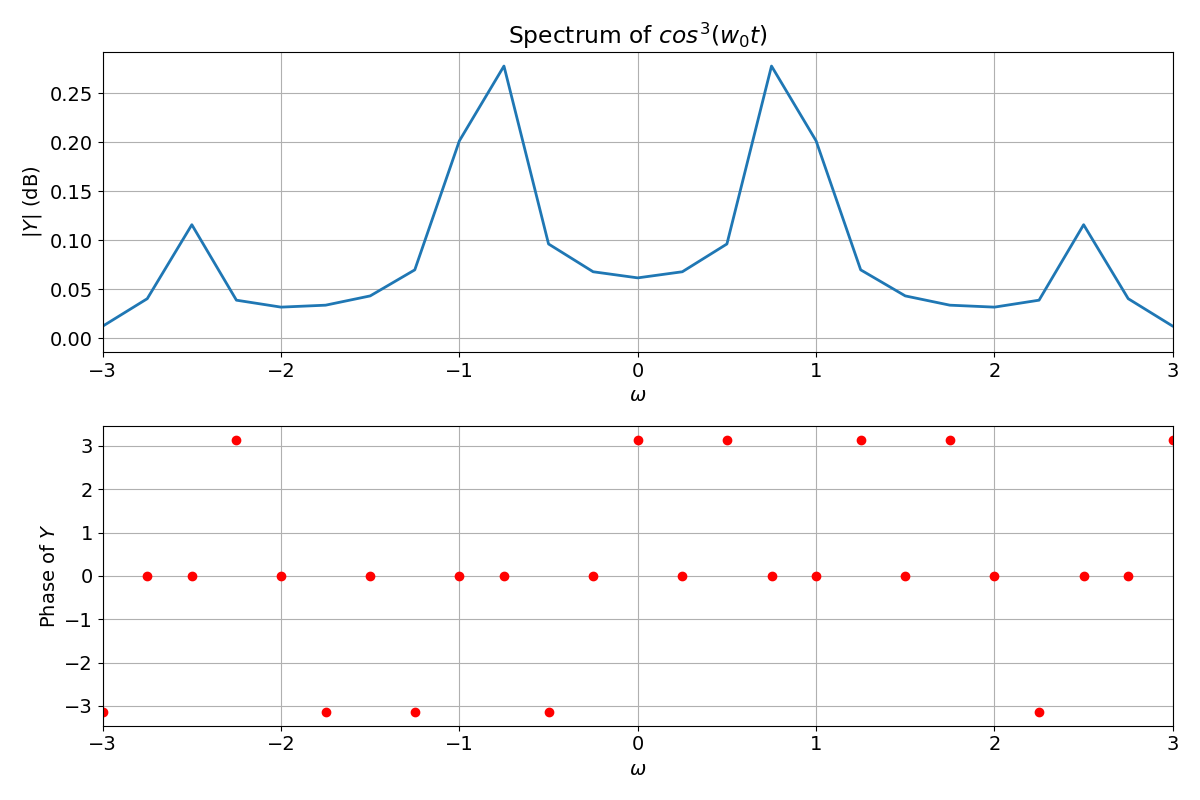
\includegraphics[scale=0.4]{plots/cos^3_wo.png}
\label{fig:8}
\end{figure}


The FFT with the hamming Window:
\begin{figure}[!tbh]
\centering
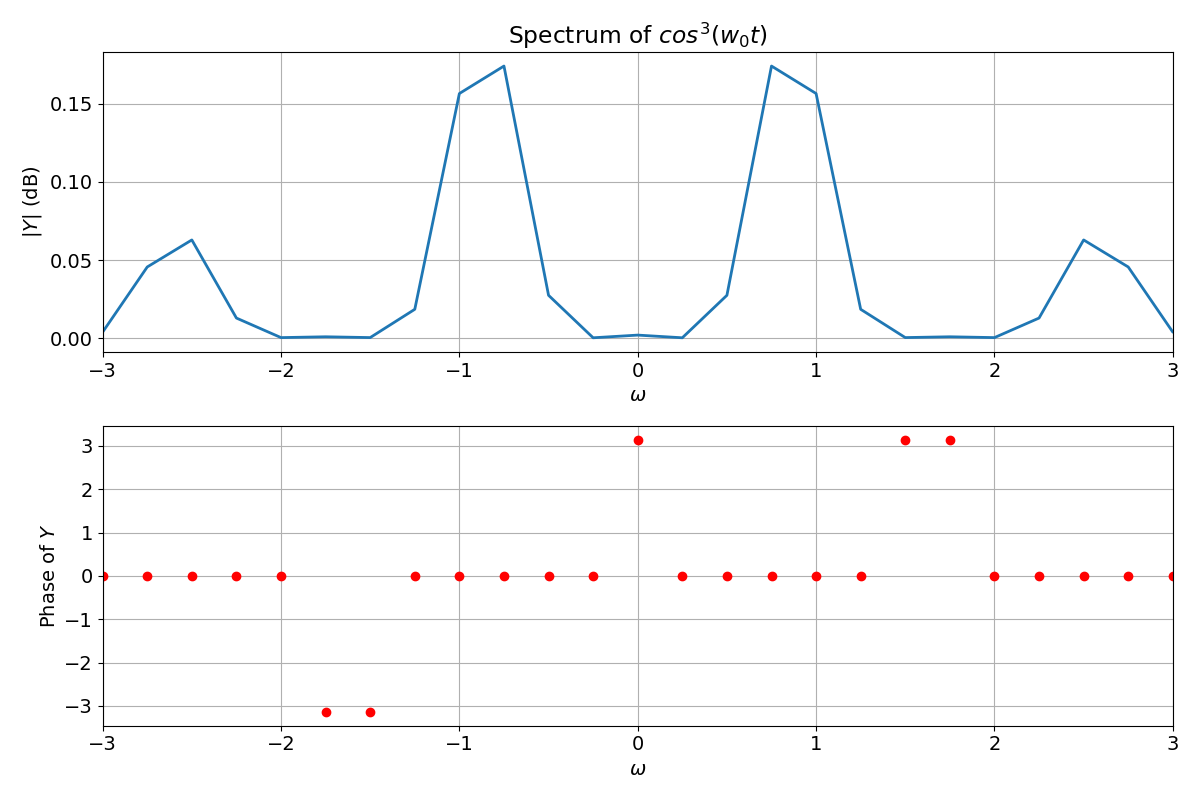
\includegraphics[scale=0.4]{plots/cos^3_with.png}
\label{fig:9}
\end{figure}

We notice that a lot of the energy is stored in frequencies that aren't a part of the signal. 
After windowing, these frequencies are attenuated and hence the peaks are sharper in the windowed function. 
It is still not an impulse because the convolution with the Fourier transform of the windowed function smears out the peak.

\subsection{Question 3}
We need to estimate $\omega$ and $\delta$ for a signal $\cos(\omega t + \delta)$ for 128 samples between $[-\pi,\pi)$. 
We estimate omega using a weighted average. We have to extract the digital spectrum of the signal and find 
the two peaks at $\pm\omega_0$, and estimate $\omega$ and $\delta$.

\begin{lstlisting}

def est_omega(w,Y):
    ii = where(w>0)
    omega = (sum(abs(Y[ii])**2*w[ii])/sum(abs(Y[ii])**2))#weighted average
    print ("omega = ", omega)

def est_delta(w,Y,sup = 1e-4,window = 1):
    ii_1=np.where(np.logical_and(np.abs(Y)>sup, w>0))[0]
    np.sort(ii_1)
    points=ii_1[1:window+1]
    print ("delta = ",np.sum(np.angle(Y[points]))/len(points))#weighted average for first 2 points

\end{lstlisting}

\begin{figure}[!tbh]
\centering
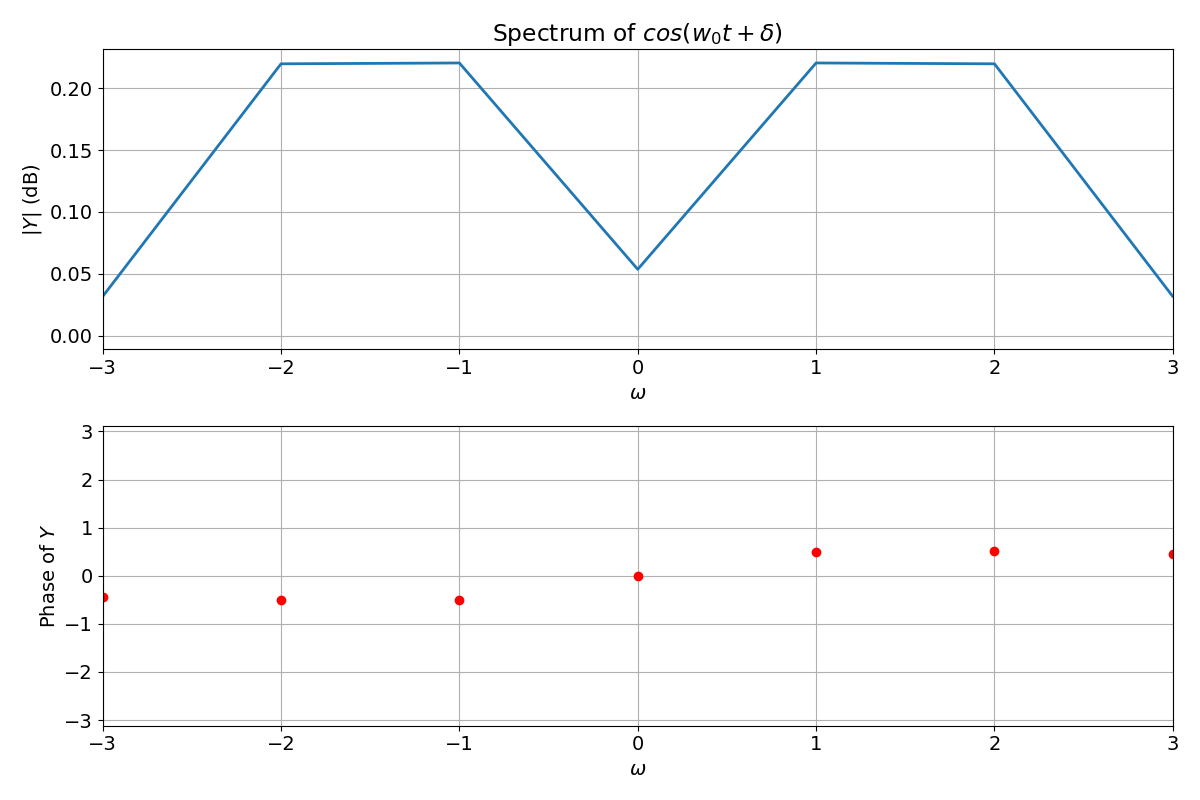
\includegraphics[scale=0.4]{plots/normal_cosine.png}
\caption{Fourier transform of $cos(1.5t+0.5)$}
\label{fig:10}
\end{figure}

\noindent
We estimate omega by performing a Mean average of $\omega$ over the magnitude of $|Y(j\omega)|$.

\noindent
For delta we consider a widow on each half of $\omega$ (split into positive and negative values) and extract their mean slope. 
The intuition behind this is that, a circular shift in the time domain of a sequence results in the linear phase of the spectra.


\subsection{Question 4}

We repeat the exact same process as question 3 but with noise added to the original signal.

\begin{figure}[!tbh]
\centering
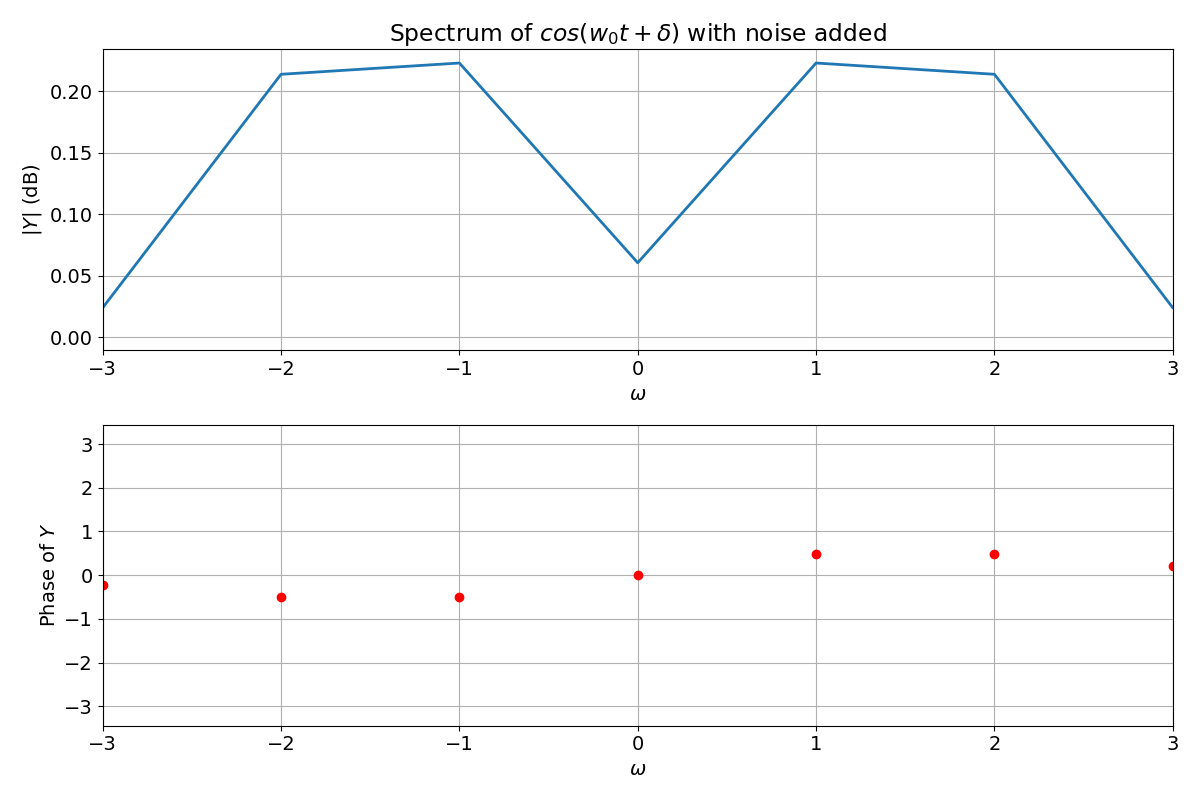
\includegraphics[scale=0.4]{plots/noisy_cosine.png}
\caption{Fourier transform of noise + $cos(1.5t+0.5)$}
\label{fig:11}
\end{figure}

\noindent
For true value of $\omega$ and $\delta$ = 1.5 and 0.5 respectively 

\begin{verbatim}

Estimating omega and delta for normal cosine: 
omega =  1.5163179648582412
delta =  0.506776265719626

Estimating omega and delta for noisy cosine: 
omega =  2.1933319678753134
delta =  0.48816479786629235

\end{verbatim}
    
\subsection{Question 5}
In this question we analyze a chirp signal which is an FM signal where frequency is directly proportional to time.
A chirp signal we shall consider is given by 
\begin{equation}
    f(t) = cos(16t(1.5 + \frac{t}{2\pi}))
\end{equation}

The FFT of the chirp is given by:
We note that the frequency response is spread between 5-50 rad/s. A large section of this range apears due to Gibbs phenomenon. 

\begin{figure}[!tbh]
\centering
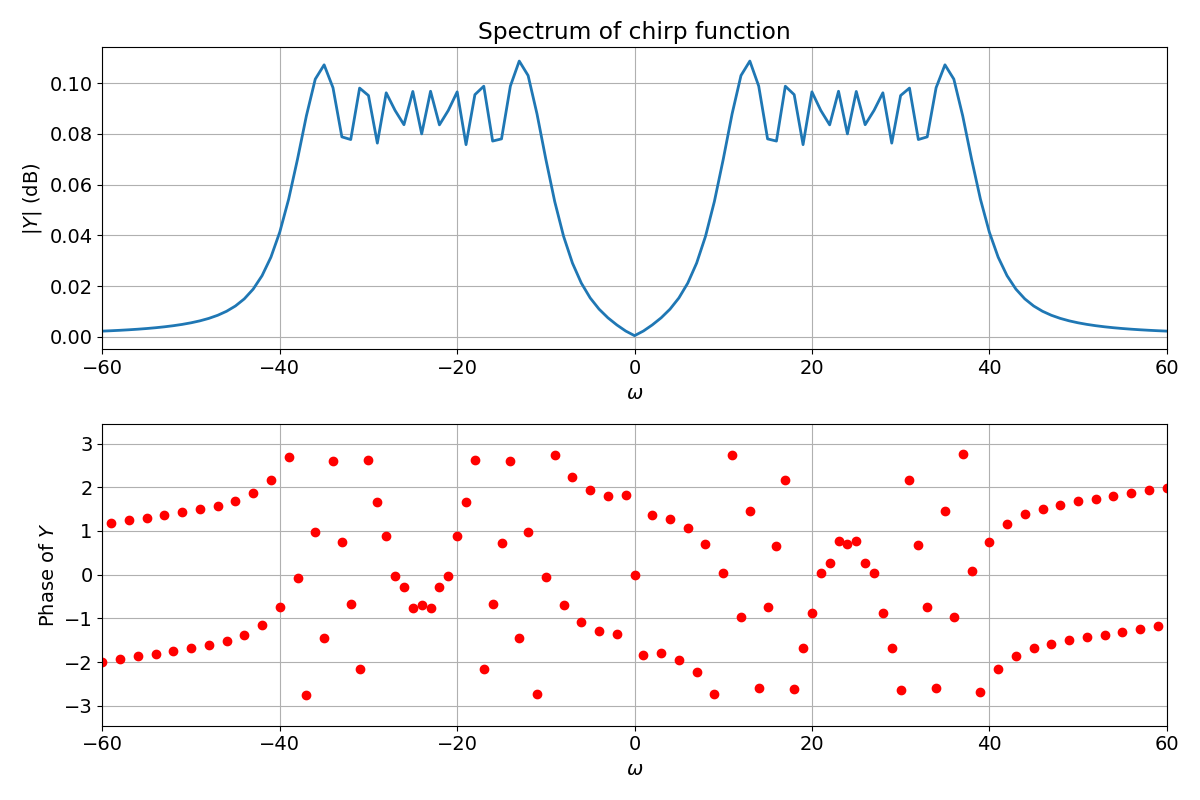
\includegraphics[scale=0.4]{plots/chirp_wo.png}
\caption{Chirp function non-windowed}
\label{fig:12}
\end{figure}

On windowing, only frequencies between 16 and 32 rad/s remain.


\begin{figure}[!tbh]
\centering
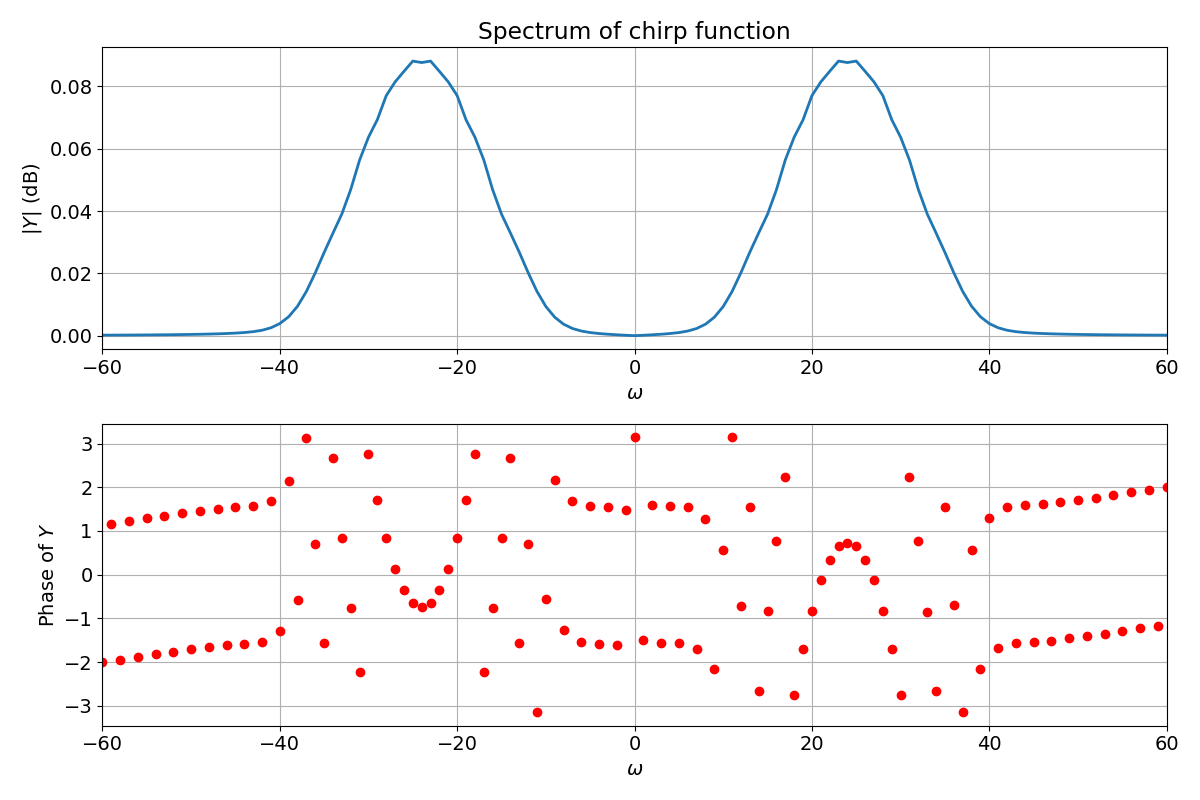
\includegraphics[scale=0.4]{plots/chirp_with.png}
\caption{Chirp function windowed}
\label{fig:13}
\end{figure}

\newpage
\subsection{Question 6}
For the same chirped signal, we break the 1024 vector into pieces that are 64 samples wide.
Extract the DFT of each and store as a column in a 2D array. Then plot the array as a surface plot to show how the frequency of the signal varies with time.
This is new. So far we worked either in time or in frequency. But this is a “time- frequency” plot, where we get localized DFTs and show how the spectrum evolves in time.
We do this for both phase and magnitude. Let us explore their surface plots. \\

\noindent
\textbf{
Surface Plots for Non Windowed Chirp Functions}

\begin{figure}[!tbh]
\centering
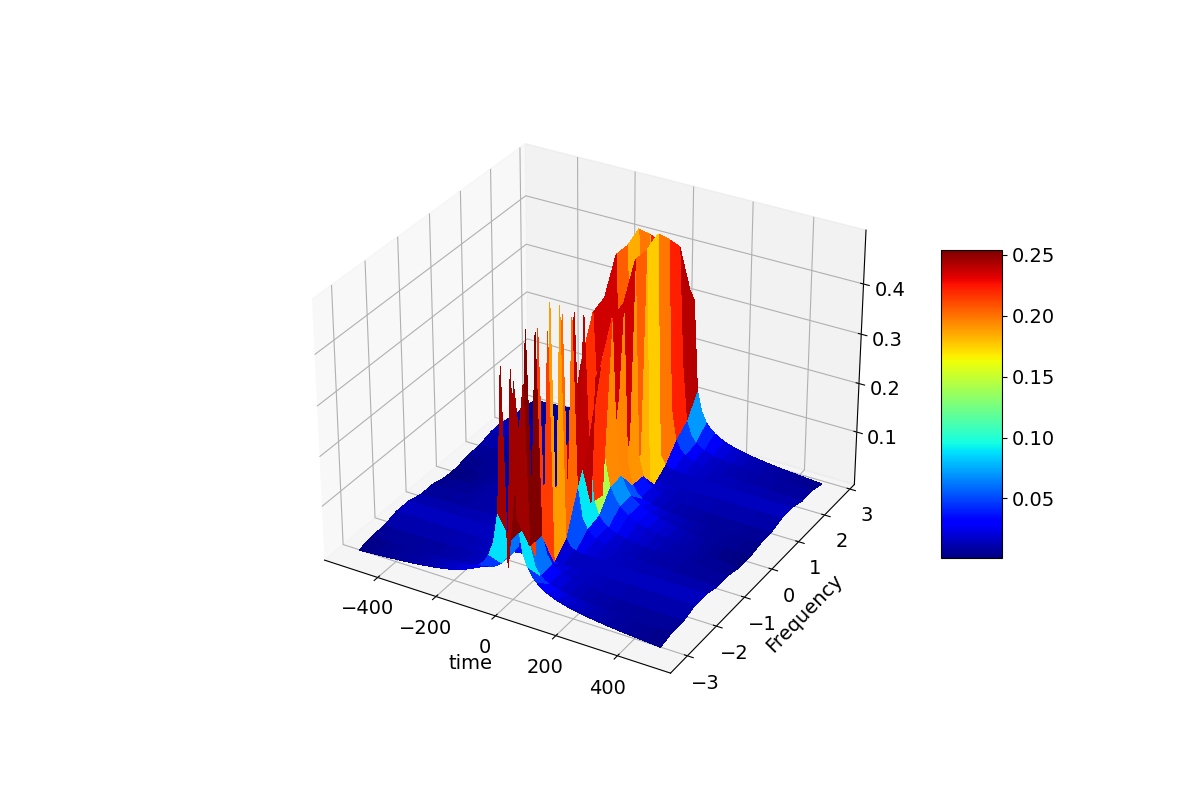
\includegraphics[scale=0.4]{plots/non_windowed_surfacemag.png}
\caption{Non Windowed Chopped Chirp function, |Fourier transform|}
\label{fig:14}
\end{figure}

\begin{figure}[!tbh]
\centering
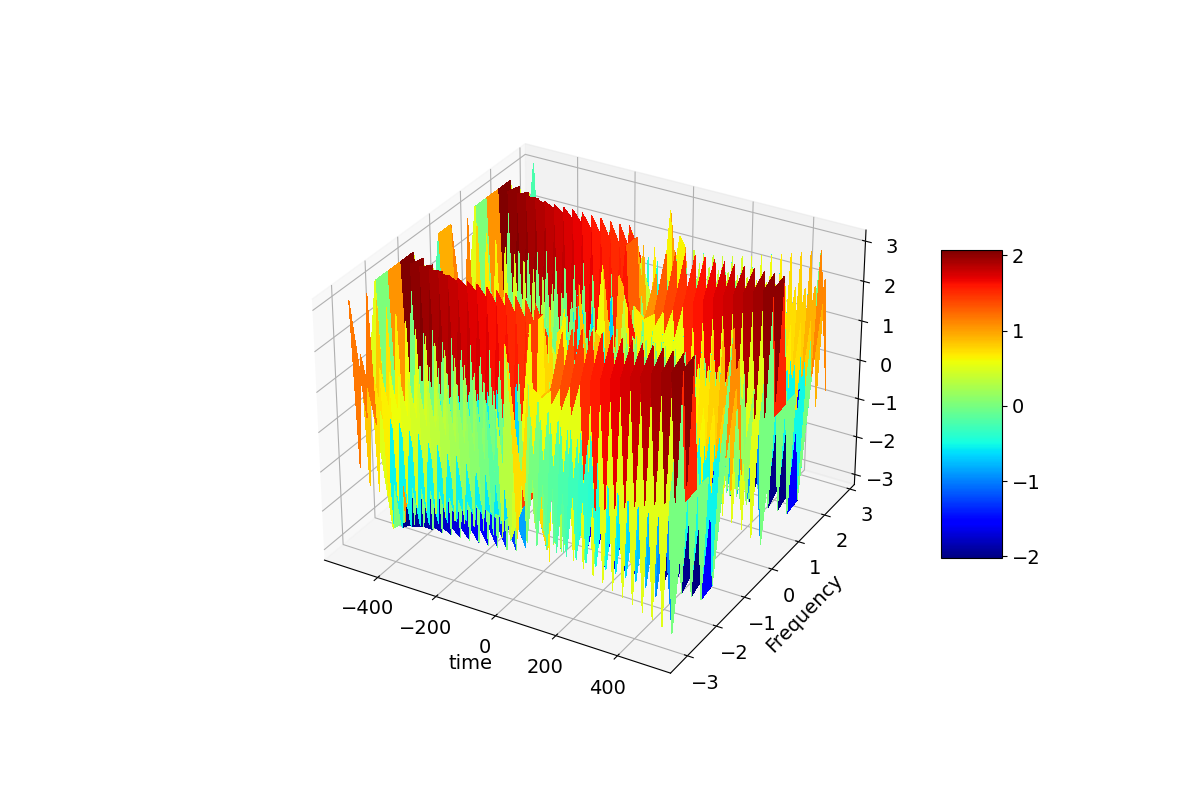
\includegraphics[scale=0.4]{plots/non_windowed_surfaceangles.png}
\caption{Chopped Chirp function, Phase of Fourier transform}
\label{fig:15}
\end{figure}
\newpage

\noindent
\textbf{
Surface Plots for Windowed Chirp Functions}

\begin{figure}[!tbh]
\centering
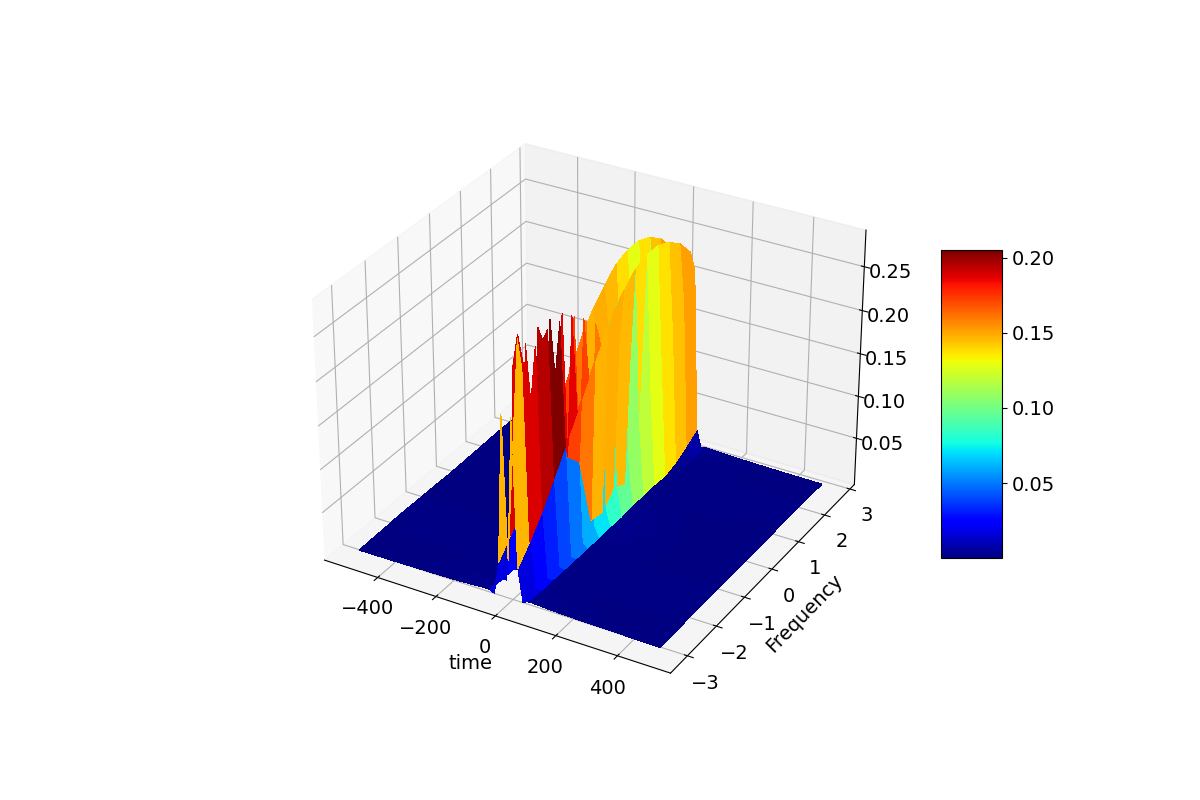
\includegraphics[scale=0.4]{plots/windowed_surfacemag.png}
\caption{Windowed Chopped Chirp function, |Fourier transform|}
\label{fig:16}
\end{figure}

\begin{figure}[!tbh]
\centering
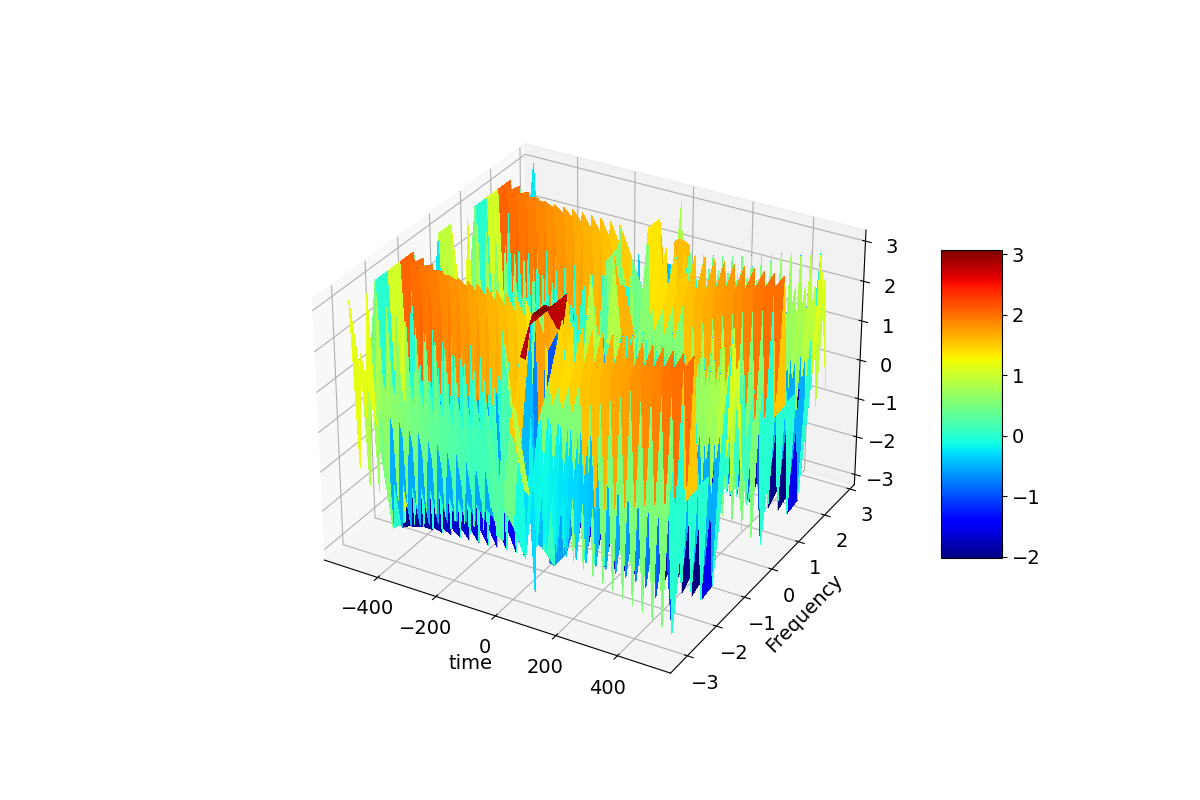
\includegraphics[scale=0.4]{plots/windowed_surfaceangles.png}
\caption{Windowed Chopped Chirp function, Phase of Fourier transform}
\label{fig:17}
\end{figure}

\newpage

\section{Conclusion}
\begin{itemize}
    \item
      From the above examples, it is clear that using a Hamming window
      before taking a DFT helps in reducing the effect of Gibbs phenomenon
      arising due to discontinuities in periodic extensions.
    \item
      However, this comes at the cost of spectral leakage. This is basically
      the blurring of the sharp peaks in the DFT. It occurs because of
      convolution with the spectrum of the windowing function. Deltas in the
      original spectrum are smoothed out and replaced by the spectrum of the
      windowing function.
    \item
      We used this windowed DFT to estimate the frequency and phase of an
      unknown sinusoid from its samples.
    \item
      By performing localized DFTs at different time isntants, we obtained a
      time-frequency plot which allowed us to better analyse signals with
      varying frequencies in time.
    \end{itemize}
    

\end{document}




